%!TEX root = main.tex

\section{Decision procedure} \label{sec:decision}

In this section, we are going to show the main result of this paper.

\begin{theorem}\label{thm-main}
The path feasibility of $\strline_{\sf reg}$ is decidable.
\end{theorem}

The proof of Theorem~\ref{thm-main} is obtained by first showing that both $\extract$ and $\replaceall$ functions can be transformed into PSST, then computing the pre-images of regular languages under PSSTs and removing all the assignment statements, finally solving the nonemptiness of intersection of regular languages. The aforementioned procedure extends the approach of backward reasoning proposed in \cite{CCH+18,CHL+19} in the following sense: While \cite{CCH+18,CHL+19} used the standard one-way/two-way transducers, we introduce a new model of PSSTs to capture the semantics of $\extract$ and $\replaceall$, where priorities are used to model the greedy/non-greedy semantics of capturing groups and string variables are used to model the back references. Moreover, as we have shown in Theorem~\ref{theorem:psst_preimage}, the pre-images of regular languages under PSSTs are still regular and can be computed effectively.

In the sequel, we shall show that semantically equivalent PSSTs can be effectively constructed from the $\extract$ and $\replaceall$ functions. 

\begin{lemma}\label{lem-extract}
From $\extract_{i,e}(x)$, a PSST $\cT_{\extract_{i,e}}$ can be constructed such that $\cR_{\cT_{\extract_{i,e}}} = \{(w, w') \mid w'= \extract_{i,e}(w)\}$.
\end{lemma}

\begin{lemma}\label{lem-replace}
From $\replaceall_{\pat, \rep}(x)$, a PSST $\cT_{\replaceall_{\pat, \rep}}$ can be constructed such that $\cR_{\cT_{\replaceall_{\pat, \rep}}} = \{(w, w') \mid w'= \replaceall_{\pat, \rep}(w)\}$.
\end{lemma}

With Lemma~\ref{lem-extract}-\ref{lem-replace}, the path feasibility of $\strline_{\sf reg}$ is reduced to the path feasibility of string-manipulating programs that are a sequential composition of the statements of the form $z:=x \concat y$, $y:=\cT(x)$ and $\ASSERT{x \in \cA}$, where $\cT$ is a PSST and $\cA$ is an FA. Let us use  $\strline'_{\sf reg}$ to denote the class of such programs. Then we can follow the backward reasoning approach of the OSTRICH solver proposed in \cite{CCH+18,CHL+19} and solve the path feasibility of $\strline'_{\sf reg}$ by repeating the following procedure, until no more assignment statements are left:\\
Let $S$ be the current $\strline'_{\sf reg}$ program.
\begin{itemize}
\item If the last assignment statement of $S$ is $y:=\cT(x)$, then let $\ASSERT{y \in \cA_1}, \cdots, \ASSERT{y \in \cA_n}$ be an enumeration of all the assertion statements for $y$ in $S$. Compute $\cR^{-1}_\cT(\Lang(\cA_1))$ as an FA $\cB_1$, $\cdots$, and $\cR^{-1}_\cT(\Lang(\cA_n))$ as $\cB_n$. Remove  the assignment  $y:=\cT(x)$ and add the assertion statements $\ASSERT{x \in \cB_1}$; $\cdots$; $\ASSERT{x \in \cB_n}$. 
%
\item If the last assignment statement of $S$ is $z:=x \concat y$, then let $\ASSERT{z \in \cA_1}, \cdots, \ASSERT{z \in \cA_n}$ be an enumeration of all the assertion statements for $z$ in $S$. Compute $\concat^{-1}(\Lang(\cA_1))$, the pre-image of $\concat$ under $\Lang(\cA_1)$, as a collection of FA pairs $(\cB_{1,j}, \cC_{1,j})_{j \in [m_1]}$, $\cdots$, and $\concat^{-1}(\Lang(\cA_n))$ as $(\cB_{n, j}, \cC_{n,j})_{j \in [m_n]}$ (c.f. \cite{CHL+19}). Remove the assignment $z:=x \concat y$, nondeterministically choose the indices $j_1 \in [m_1], \cdots, j_n \in [m_n]$, and add the assertion statements $\ASSERT{x \in \cB_{1,j_1}}; \ASSERT{y \in \cC_{1, j_1}}$; $\cdots$; $\ASSERT{x \in \cB_{n,j_n}}; \ASSERT{y \in \cC_{n, j_n}}$. 
\end{itemize}

It remains to show Lemma~\ref{lem-extract} and Lemma~\ref{lem-replace}. As a preparation, we first show how a PFA can be constructed from $e \in \regexp[\sf CG]$. Then we prove the two lemmas. 


\subsection{From $\regexp[\sf CG]$ to PFA}
\label{construction:pnfa}

\begin{figure*}
	\centering
	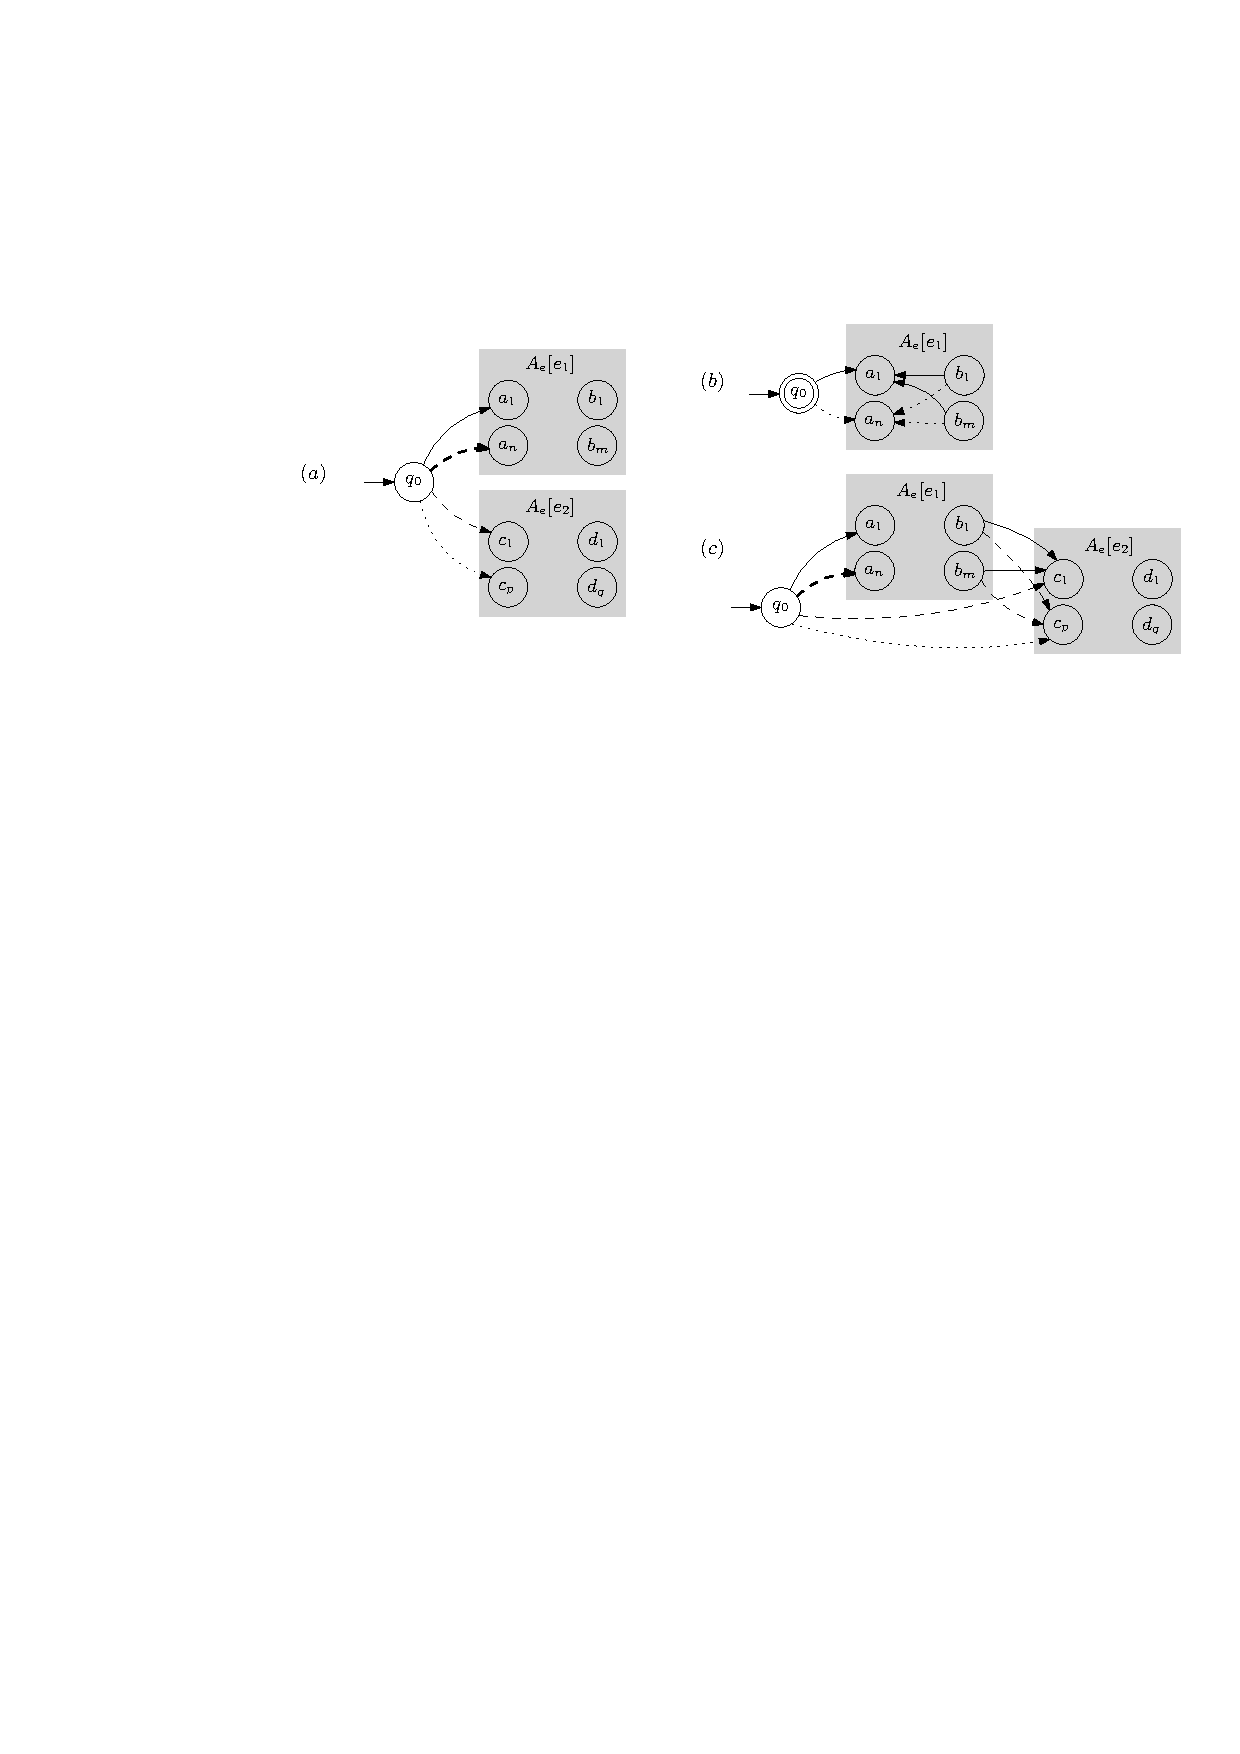
\includegraphics{pglushkov_01}
	\caption{pNFA $A_e$ for (a) $e=e_1+e_2$ (b) $e=e_1^{\ast}$ and (c) $e=e_1 \concat e_2$ where $\varepsilon \in \Lang(e_1)$ and $\varepsilon \notin \Lang(e_2)$. A transition of lower priority is depicted thiner and more densely dotted. }
	\label{fig:pglushkov}
\end{figure*}

For any $e \in \regexp[\sf CG]$, we define a pNFA $A_e$ by an adaptation of the standard
Glushkov construction \cite{Gluskov61}. The original construction on regular expressions
produces an FA without $\varepsilon$-transitions, which we denote by $G_e$.
%The state of $G_e$ comprises $q_0$ which is a special starting state, and $a_i$'s
%where the $i$-th character occurring in e is $a$. 
We refer the reader to \cite{Gluskov61} for 
details of how to construct $G_e$. %\tl{is this just the textbook construction?}

The pNFA $A_e$ is obtained by recursively adding priority to $G_e$ as follows:
\begin{itemize}
  \item If $e = \varepsilon$ or $e = a$ or $e = \emptyset$, then $A_e = G_e$.
  
  \item If $e = (e_1)$, then $A_e = A_{e_1}$.
  
  \item If $e = e_1 + e_2$, and suppose $A_{e_1} = (\{ q_0 \} \cup Q_1,
  \Sigma, \delta_1, q_0, F_1)$ and $A_{e_2} = (\{ q_0 \} \cup Q_2, \Sigma,
  \delta_2, q_0, F_2)$, then $A_e = (\{ q_0 \} \cup Q_1 \cup Q_2, \Sigma,
  \delta, q_0, F_1 \cup F_2)$, where $\delta$ is defined by following rules:
  \begin{itemize}
    \item for any $q \neq q_0$, $a \in \Sigma$ and $q_1 \ldots q_n \in
    \overline{Q_{_1}} \cup \overline{Q_2}$ such that $\delta_1 (q, a) = q_1
    \ldots q_n$ or $\delta_2 (q, a) = q_1 \ldots q_n$, we have $\delta (q, a)
    = q_1 \ldots q_n$
    
    \item for any $a \in \Sigma$, if $\delta_1 (q_0, a) = q_1 \ldots q_n$ and
    $\delta_2 (q_0, a) = q'_1 \ldots q'_m$, then $\delta (q_0, a) = q_1 \ldots
    q_n q'_1 \ldots q'_m$
  \end{itemize}
  \item If $e = e_1 e_2$, and suppose $A_{e_1} = (\{ q_0 \} \cup Q_1, \Sigma,
  \delta_1, q_0, F_1)$ and $A_{e_2} = (\{ q_0 \} \cup Q_2, \Sigma, \delta_2,
  q_0, F_2)$, then $A_e = (\{ q_0 \} \cup Q_1 \cup Q_2, \Sigma, \delta, q_0,
  F)$, where $F$ is defined as:
  \[ F = \left\{ \begin{array}{ll}
       F_1 \cup F_2 & \varepsilon \in L (e_1) \wedge \varepsilon \in L (e_2)\\
       (F_1 \cup F_2) \backslash \{ q_0 \} & \varepsilon \nin L (e_1) \wedge
       \varepsilon \in L (e_2)\\
       F_2 & \varepsilon \nin L (e_2)
     \end{array} \right. \]
  and $\delta$ is defined by following rules:
  \begin{itemize}
    \item For any $q \in (Q_1 \cup Q_2) \backslash F_1$, $a \in \Sigma$ and
    $q_1 \ldots q_n \in \overline{Q_{_1}} \cup \overline{Q_2}$ such that
    $\delta_1 (q, a) = q_1 \ldots q_n$ or $\delta_2 (q, a) = q_1 \ldots q_n$,
    we have $\delta (q, a) = q_1 \ldots q_n$
    
    \item For any $q \in F_1 \backslash \{ q_0 \}$, $a \in \Sigma$, if
    $\delta_1 (q, a) = q_1 \ldots q_m$ and $\delta_2 (q_0, a) = q_1' \ldots
    q_n'$, then we have $\delta (q, a) = q_1 \ldots q_m q_1' \ldots q_n'$.
    
    \item For any $a \in \Sigma$, suppose $\delta_1 (q_0, a) = q_1 \ldots q_m$
    and $\delta_2 (q_0, a) = q_1' \ldots q_n'$. If $q_0 \in F_1$, then $\delta
    (q_0, a) = q_1 \ldots q_m q_1' \ldots q_n'$. If not, $\delta (q_0, a) =
    q_1 \ldots q_m$.
  \end{itemize}
  \item If $e = e_1^{\ast}$, and suppose $A_{e_1} = (\{ q_0 \} \cup Q_1,
  \Sigma, \delta_1, q_0, F_1)$, then $A_e = (\{ q_0 \} \cup Q_1, \Sigma,
  \delta, q_0, F)$ where $F = F_1 \cup \{ q_0 \}$ and $\delta$ is defined by
  following rules:
  \begin{itemize}
    \item For any $q \in (\{ q_0 \} \cup Q_1) \backslash \{ F_1 \}$, $a \in
    \Sigma$ and $q_1 \ldots q_n \in \overline{Q_1}$ such that $\delta_1 (q, a)
    = q_1 \ldots q_n$, we have $\delta (q, a) = q_1 \ldots q_n$
    
    \item For any $q \in F_1$ and $a \in \Sigma$, if $\delta_1 (q_0, a) = q_1
    \ldots q_m$ and $\delta_1 (q, a) = q_1' \ldots q_n'$, then for every we
    have $\delta (q, a) = q_1 \ldots q_m q_1' \ldots q_n'$.
  \end{itemize}
\end{itemize}

The key transitions of some non-trivial cases of the construction are illustrated in Figure.\ref{fig:pglushkov}.

 An important property of the automaton $G_e$ and thus $A_e$ is that, for any subexpression $e'$ of $e$, there must be a subgraph of $A_{e}$ corresponding to $e'$. We denote this subgraph by $A_{e}[e']$. This subgraph can be seen as the automaton obtained by removing from $A_{e'}$ the state $q_0$ and all transitions from it.
 
 For instance, if $e = (a (ab)^*)^*$ and $e' = a(ab)^*$, then $A_{e}[e']$ is the subgraph of $A_{e}$ comprising the states $\{a_1, a_2, b_3\}$ and the transitions $\{(a_1, a, a_2), (a_2, b, b_3), (b_3, a, a_2)\}$.
 
 Figure.\ref{fig:pglushkov} also illustrates the subgraphs corresponding to direct subexpressions of $e$.
 


\begin{definition}
  Let $A_e$ be the pNFA constructed for $e$, and $p = q_0 \sigma_1 q_1 \ldots
  \sigma_m q_m$ is the accepting run of $A_e$ on string w. For any subexpression $e'$ of $e$, we say a
  consecutive sequence of states $q_i q_{i + 1} \ldots q_{j - 1} q_j$ in p is
  a maximal $e'$-match, if $q_i \in \tmop{Start} (e')$, $q_j \in \tmop{End}
  (e')$, $(q_{i - 1}, \sigma_i, q_i)$ is not a transition in $A_e [e']$, and
  for any $k \in [i, j]$, $q_k$ is a vertex in $A_e [e']$. Moreover, if $j
  \neq m$, then $(q_j, \sigma_{j + 1}, q_{j + 1})$ is not a transition in $A_e
  [e']$.
  
  We use $p_{e', e} (w)$ to denote the sequence of disjoint maximal $e'$-match
  $w_1 \ldots w_n$, in the order they occur in p. Note that in $A_e$, all
  states except $q_0$ are labeled by a letter, thus a maximal $e'$-match can
  be seen as a string.
\end{definition}

The following  theorem states the equivalence of the accepting match of a \regexp[\sf CG] $e$ and the accepting run of $A_e$ on the same input string, thus the construction precisely captures the semantics. % in \ref{semantics:regex}.
\begin{theorem}
 \label{theorem:regex_pnfa_equiv}
  For any regular expression e, subexpression $e'$ of e, and $w \in L (e)$,
  $m_{e', e} (w) = p_{e', e} (w)$
\end{theorem}

For simplicity, we refer the reader to the appendix for proof.


 
\subsection{Proof of Lemma~\ref{lem-extract}-\ref{lem-replace}}



%%%%%%%%%%%%%%%%%%%%%%%%%%%%%%%%%%%%%%%%%%%%%%%%%%
%%%%%%%%%%%%%%%%%%%%%%%%%%%%%%%%%%%%%%%%%%%%%%%%%%
\hide{
\begin{definition}[Two way NSST?]
  The definition of 2NSST is just like 2FT, allowing bidirectional move of
  NSST's head.
\end{definition}

\begin{note}
  One thing is worth noting about this idea of 2NSST: \tmtextit{the pre-image
  of 2NSST is still computable}. We just use a 2FA N to simulate the 2NSST, in
  the same manner of the construction above. We can then transform the 2FA
  into a one-way FA in exponential time.
  
  However, the expressive power of 2NSST is unknown (yet). I highly suspect
  that 2NSST is equivalent to NSST, since the bidirectional move of head
  provides the same function as variables, to some extent. Anyway, the
  expressive power of NSST should be sufficient now.
\end{note}

All the function expressible by 2FT is also expressible by NSST, like
\tmtextit{split}. Below is an example of what more NSST can express.
}
%%%%%%%%%%%%%%%%%%%%%%%%%%%%%%%%%%%%%%%%%%%%%%%%%%
%%%%%%%%%%%%%%%%%%%%%%%%%%%%%%%%%%%%%%%%%%%%%%%%%%

%\begin{definition}[Regular Expression with capturing group, regex]
%  Suppose $\Gamma$ is some set of variables, x is an element of $\Gamma$. a is
%  a character in $\Sigma$
%  \[ \alpha \colons = \varepsilon |a| \alpha + \alpha | \alpha \circ \alpha |
%     \alpha^{\ast} | (\alpha) \%x \]
%  WLOG, we assume a variable occurs at most once in a regex.
  
%  the semantics of regex is defined as tuple $(w, w_x, w_y, \ldots)$ where w
%  is the whole string matched, and $w_x$ is the string matched by the
%  capturing group marked by x, etc. A more formal definition involves match
%  trees and recursive definition.
%  See{\cite{CSY03,CN09}}
%\end{definition}

%\begin{definition}[Semantics of $\replaceall_{\pat, \rep}$]
%  Consider the constriant $y = \replaceall_{\pat, \rep}(x)$, where $\pat \in \regexp[\sf CG]$ and $\rep \in \refexp$.
%  
%The semantics of $\replaceall_{\pat, \rep}$ is  similar to that in {\cite{CCH+18}}, where the leftmost and longest matching of
%  $e_1$ in $x$ is considered, with the difference that here the replacement string is obtained from a matching of $e_1$ by replacing every reference $\$ n$ in $e_2$ with the string matched by the subexpression corresponding to the $n$-th capturing group.
%%  
%\zhilin{A more formal definition should be added in the future.}
%\end{definition}

%\begin{remark}
%  In the aforementioned definition of the semantics of $\replaceall_{\pat,\rep}(x)$, the matching of $\pat$ in $x$ is deterministic since the leftmost and longest matching is considered, and the process of matching the subexpressions is captured by the semantics in \ref{semantics:regex}.
%  
%Therefore, the $\replaceall_{e_1,e_2}(x)$ function can be seen as a precise modeling of that used in practical programming languages, e.g. Javascript. \zhilei{might need exemplification}
%\end{remark}


\begin{theorem}
  Each $\pat \in \regexp[\sf CG]$ and $\rep \in \refexp$, $\replaceall_{\pat, \rep}$ can be modeled by a $\PSST${} $T_{e_1,e_2}$.
\end{theorem}

\begin{proof}

Suppose pNFA $A_{e_1} =(Q, \Sigma,  \delta, q_0, F)$ is the Glushkov automaton constructed from $e_1 \in \regexp[\sf CG]$ by the modified algorithm in \ref{construction:pnfa}. From the algorithm, we know that $Q$ is the union of the initial state $q_0$ and the set of $a_i$'s where the $i$-th character occurring in $e$ is $a$.

For each subexpression $e'$ of $e_1$, we use $C_{e'}$ to denote the set of subexpressions of $e'$ corresponding to a capturing group in $e'$, i.e. the set $\{v \in S(e')\mid \exists v'. v=(v')\}$.

For each state $a_i$ of $A_{e_1}$, we define $C(a_i)$  as the set $\{ e' \in C_{e_1} \mid a_i \mbox{ is a vertex in }
A_{e_1}[e']\}$. Intuitively, $C(a_i)$ represents the set of subexpressions in $C_{e_1}$ whose values should be updated when entering the state $a_i$ in $A_{e_1}$. 

Moreover, for each $e' \in C_{e_1}$, we use $\ssym(e')$ (resp. $\esym(e')$) to denote the set of marked symbols that can be matched to the first  (resp. last) symbol of a string in $\Lang(e')$. For instance, let $e' = a(ab)^*$, then $\ssym(e') = \{a_1\}$ and $\esym(e') = \{a_1, b_3\}$. 

For each $e' \in C_{e_1}$, we introduce a string variable $x_{e'}$. Besides, a special string variable $x_{res}$ is introduced to store, accumulate, and denote the result of $\replaceall_{e_1,e_2}$. Let $X$ denote the set of these string variables.


Then we construct the \PSST{} $T_{e_1,e_2} = (Q', \Sigma, X, E, \delta', q_0', F')$, by using the idea of parsing automata in \cite{CCH+18}. Note in the below, we omit the priority of some transitions and simply write $q' \in \delta'(q,a)$ instead of $\delta'(q,a)=(q_1,q_2,\ldots,q_n)$. In this case, the priority is immaterial and any combination will work.

At first, $q'_0= (\{ q_0
\}, \tmop{left}, \emptyset)$. The set of transition rules $\delta'$ is defined by the following rules.

\begin{itemize}
  
  \item Suppose $(\rho \{ q_0 \}, \tmop{left}, S) \in Q'$, $a \in \Sigma$,
  $\delta (S, a) \cap F = \emptyset$ and $\delta^{\ast} (\rho \{ q_0 \}, a) \cap F =
  \emptyset$, then
  \[ (\tmop{red} (\delta^{\ast} (\rho \{ q_0 \}, a)) \{ q_0 \}, \tmop{left}, \delta
     (S, a)) \in \delta' ((\rho \{ q_0 \}, \tmop{left}, S), a) \]
  and the corresponding assignment is defined as $s(x_{res}) = res \concat a$ and $s(x_{e'})=x_{e'}$ for
  every $e' \in C_{e_1}$.
  
  \item Suppose $(\rho \{ q_0 \}, \tmop{left}, S) \in Q'$ and $a \in \Sigma$.
  If $\delta (S, a) \cap F = \emptyset$, $\delta^{\ast} (\rho, a) \cap F = \emptyset$
  and $\delta (q_0, a) \nsubseteq \delta (S, a) \cup \delta^{\ast} (\rho, a)$, then
  for every $q' \in \delta (q_0, a) \backslash \delta (S, a) \cup \delta^{\ast}
  (\rho, a)$, we have
  \[ (\{ q' \}, \tmop{long}, \delta (S, a) \cup \delta^{\ast} (\rho, a)) \in \delta'
     ((\rho \{ q_0 \}, \tmop{left}, S), a) \]
  and $s$ is the assignment function defined as follows: $s(x_{e'}) = a$ for every $e'  \in C(q')$, and $s(y)=y$ for every other string variable $y \in X$.
  
  \item Suppose $(\{ q \}, \tmop{long}, S) \in Q',$ and $a \in \Sigma$. If
  $\delta (S, a) \cap F = \emptyset$, $\delta (q, a) \nsubseteq \delta (S,
  a)$, and $\delta (q, a) \backslash \delta (S, a) = \{ q_1, \ldots,
  q_n \}$, where $\delta (q, a) = \ldots q_i \ldots q_j \ldots$ for all $i < j$,
  we have $\forall i \in [n]$
  \[ (\{ q_i \}, \tmop{long}, \delta (S, a)) \in \delta' ((\{ q \},
     \tmop{long}, S), a) \]
  and the transition to $(\{ q_i \}, \tmop{long}, \delta (S, a))$ is more prioritized than the transition to
  $(\{ q_j \}, \tmop{long}, \delta (S, a))$ for all $i < j$. 
  
  For any $i \in [n]$, the corresponding assignment $s_i$ is defined as follows:
  
  Suppose $\Theta = \{e' \mid e' = e''^*  \wedge
  q \in \esym(e'') \wedge q_i \in \ssym(e'') \}$ and $C_{\Theta}$ denotes the set of subexpression $e''$ such that $e'' \in C_{e'}$ for some $e' \in \Theta$.
Then 
\begin{itemize}
\item for each $e \in C_{\Theta} \cap C(q_i)$, $s(x_e) = a$,
%
\item for each $e \in C_{\Theta} \setminus C(q_i)$, $s(x_e) = \varepsilon$, 
%
\item for each $e \in C(q_i) \setminus C_\Theta$, $s(x_e) = x_e \concat a$,
%
\item for each $e \in X \setminus (C_\Theta \cup C(q_i))$, $s(x_e)= x_e$.
\end{itemize}

    \item Suppose $(\{ q \}, \tmop{long}, S) \in Q'$, and $a \in \Sigma$. If
  $\delta (S, a) \cap F = \emptyset$, and $\delta (q, a) \cap F = \{ q_1,
  \ldots, q_n \}$, where $\delta (q, a) = \ldots q_i \ldots q_j \ldots$ for all
  $i < j$, we have $\forall i \in [n]$,
  \[ (\{ q_0 \}, \tmop{left}, \delta (S, a) \cup \{ q_i \}) \in \delta' ((\{ q
     \}, \tmop{long}, S), a) \]
  and the transition to $(\{ q_0 \}, \tmop{left}, \delta (S, a) \cup \{ q_i \})$ is more
  prioritized than the transition to $(\{ q_0 \}, \tmop{left}, \delta (S, a) \cup \{ q_j \})$
  for all $i < j$.
  
  For every $i \in [n]$, the corresponding assignment $s_i$ is defined as follows:
  
  Suppose $\Theta = \{e' \mid e' = e''^*  \wedge
  q \in \esym(e'') \wedge q_i \in \ssym(e'') \}$ and $C_{\Theta}$ denotes the set of $e''$ such that $e'' \in C_{e'}$ for some $e' \in \Theta$. Then $s (x_{res}) = x_{res}  \concat b_1   \ldots  b_n$ such that $e_2 = a_1 \ldots a_n$, and for each $i \in [n]$, if $a_i  \in \Sigma$, then $b_i = a_i$, otherwise, $a_i = \$ j$ for some $j$, let $e' \in C_{e_1}$ be the subexpression corresponding to the $j$-th capturing group of $e_1$, then:
  
  \begin{itemize}
\item if $e' \in C_{\Theta} \cap C(q_i)$, $b_j = a$,
%
\item if $e' \in C_{\Theta} \setminus C(q_i)$, $b_j = \varepsilon$, 
%
\item if $e' \in C(q_i) \setminus C_\Theta$, $b_j= x_{e'} \concat a$,
%
\item if $e' \in X \setminus (C_\Theta \cup C(q_i))$, $b_j = x_{e'}$.
\end{itemize}
  
  Moreover, $s(y) = \varepsilon$ for every other variable $y \in X$
  
  \item Suppose $(\rho \{ q_0 \}, \tmop{left}, S) \in Q'$, $a \in \Sigma$,
  $\delta (S, a) \cap F = \emptyset, \delta^{\ast} (\rho, a) \cap F = \emptyset,
  \delta (q_0, a) \cap F = \{ q_1, \ldots, q_n \}$ where $\delta (q, a) =
  \ldots q_i \ldots q_j \ldots$ for all $i < j$. We have for every $i \in [n],$
  \[ (\{ q_0 \}, \tmop{left}, \delta (S, a) \cup \delta^{\ast} (\rho, a) \cup \{ q_i
     \}) \in \delta' ((\rho \{ q_0 \}, \tmop{left}, S), a) \]
  and the transition to $(\{ q_0 \}, \tmop{left}, \delta (S, a) \cup \delta^{\ast} (\rho, a) \cup \{
  q_i \})$ is more prioritized than the transition to $(\{ q_0 \}, \tmop{left}, \delta (S, a)
  \cup \delta^{\ast} (\rho, a) \cup \{ q_j \})$ for all $i < j$.
  
  For every $i \in [n]$, the corresponding assignment $s_i$
  is defined as:
  
  $s (x_{res}) = x_{res}  \concat b_1   \ldots  b_n$ such that $e_2 = a_1 \ldots a_n$, and for each $i \in [n]$, if $a_i  \in \Sigma$, then $b_i = a_i$, otherwise, $a_i = \$ j$ for some $j$, let $e' \in C_{e_1}$ be the subexpression corresponding to the $j$-th capturing group of $e_1$, then if $e' \in C(q_i)$, $b_j = a$, otherwise $b_j = \varepsilon$

  Moreover, $s(y) = \varepsilon$ for every other variable $y \in X$
  
\end{itemize}
The output function $F'$ is simple: $F' (q) = x_{res}$  iff $q = (-, \tmop{left}, -) $.
\end{proof}

\subsection{Complexity}

\begin{proposition}[POPL'19]
	The path feasibility problem of the following two fragments is non-elementary: SL with 2FTs, and SL with FTs+replaceAll.
	
	SL[conc, replaceAll, reverse, FFT] is expspace-complete (note that 2FTs in SL are restricted to be one-way and functional)
\end{proposition}

%The same proof strategy can be used for FTs+replaceAll. The 2FTs used in the proof above
%proceed by running completely over the word and producing some output, then silently moving
%back to the beginning of the word. An arbitrary number of passes are made in this way. We
%can simulate this behaviour using FTs and replaceAll.


The main open question is the complexity of the SL fragment with replaceall function and prioritized streaming transducers. Note that PSST can simulate 2FT (adapting Matt's proof?), so we could obtain nonelementary lower bound for SL with PSST.

However, this variant of replaceall is quite different from the replaceall we had before ...

\begin{enumerate}
\item  does  copyless help?
\item how about SL with only this version of replaceall?
\end{enumerate}
